% Simulation approaches versus abstraction levels
% Author: Valeria Borodin
\documentclass[border=10pt,svgnames]{standalone} 
%%%<
\usepackage{verbatim}
%%%>
\begin{comment}
:Title: Simulation approaches versus abstraction levels
:Tags: Diagrams;Shadows;Styles
:Author: Valeria Borodin
:Slug: simulation-abstraction

This is the LaTeX version of the figure from the following link:
https://en.wikipedia.org/wiki/AnyLogic#/media/File:Simulation_approaches_vs_abstraction_levels.jpg
Note that the color range is slightly modified.

This example illustrates how modelling approaches correspond
to the abstraction levels.
\end{comment}
\usepackage{tikz}
\usetikzlibrary{positioning,shadows.blur}
\usepackage{pifont}
\renewcommand{\labelitemi}{\ding{112}}
\begin{document}

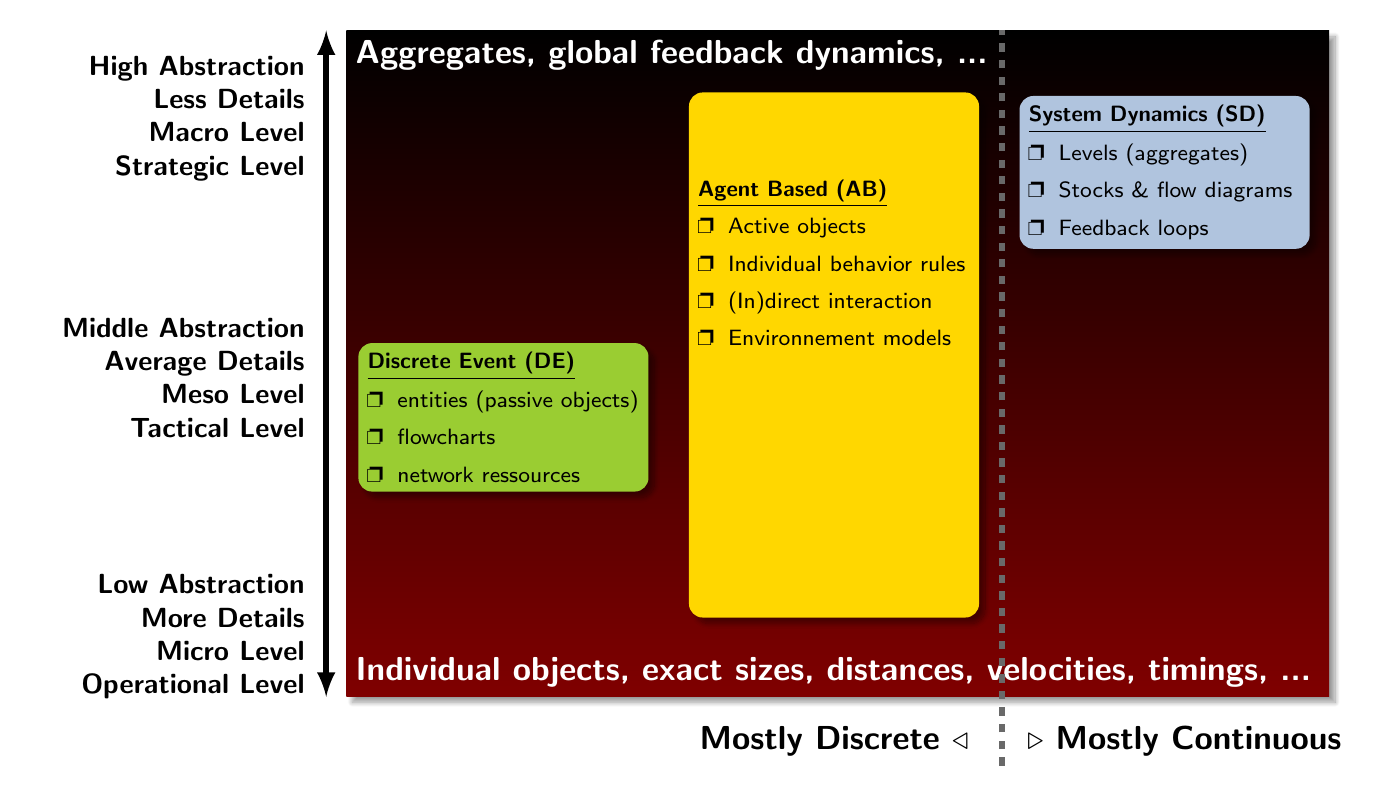
\begin{tikzpicture} 
   \tikzset{
     box/.style    = { rounded corners = 5pt,
                       align           = left,
                       font            = \sffamily\footnotesize,
                       text width      = 3.45cm, 
                       blur shadow     = {shadow blur steps = 15} },    
     legend/.style = { font       = \sffamily\bfseries, 
                       align      = right,
                       text width = 3.4cm},
  }
  \node [shade,
    blur shadow  = {shadow blur steps = 15},
    text width   = 1.01\textwidth,
    top color    = black, 
    bottom color = Maroon,
    text         = white, 
    font         = \sffamily\bfseries\large] (A)
    {Aggregates, global feedback dynamics, ...  \\ \vspace{.6\textwidth} 
    Individual objects, exact sizes, distances, velocities, timings, ...};
  
  \node [box, below left  = -4.5cm and -3.85cm of A, fill = YellowGreen]
    (DE)
    {\underline{\bfseries Discrete Event (DE)}
      \begin{itemize} 
        \setlength{\itemindent} {-.5cm}
        \item entities (passive objects)
        \item flowcharts 
        \item network ressources
      \end{itemize}
    };

  \node [box, above right  = -3.5cm and .5cm of DE,
    minimum height=0.55\textwidth, fill = Gold, text depth = 0.35\textwidth]
    (AB)
    { \underline{\bfseries Agent Based (AB)} 
        \begin{itemize} \setlength{\itemindent}{-.5cm}
          \item Active objects
          \item Individual behavior rules
          \item (In)direct interaction
          \item Environnement models
          \end{itemize}  
    };

  \node [box, above right  = -2.cm and .5cm of AB, fill = LightSteelBlue]
    (SD)
    { \underline{\bfseries System Dynamics (SD)}
      \begin{itemize} \setlength{\itemindent}{-.5cm}
        \item Levels (aggregates)
        \item Stocks \& flow diagrams
        \item Feedback loops
      \end{itemize}
    };

  \node [legend, above left = -1.25cm and 4.75cm of AB] (HA)
    {High Abstraction \\ Less Details \\ Macro Level \\ Strategic Level};

  \node [legend, below = 1.5cm of HA] (MA)
    {Middle Abstraction \\ Average Details \\ Meso Level \\ Tactical Level};
  
  \node [legend, below = 1.5cm of MA] (LA)
    {Low Abstraction \\ More Details \\ Micro Level \\ Operational Level};

  \node [below = 1.25cm of AB, font = \sffamily\bfseries\large ] (d1) 
    {Mostly Discrete $\triangleleft$};

  \node [right = .5cm of d1, font = \sffamily\bfseries\large ] (d2) 
    {$\triangleright$ Mostly Continuous };
  
   \path [ draw, color = DimGray, dashed, line width = 2pt ]
     (d1.south east) + (0.3cm,0)   coordinate(x1) -- (x1|-A.north);  
   
   \path [draw, <->, >=latex, line width = 2pt ]
     (A.south west)  + (-0.25cm,0) coordinate(x2) -- (x2|-A.north);
\end{tikzpicture}
\end{document}